% !TeX encoding = utf-8
% !TeX program = pdflatex

% !Mode:: "TeX:UTF-8"
%%  本模板可以使用以下两种方式编译:
%%
%%     1. PDFLaTeX[推荐]
%%     2. XeLaTeX

%%  注意:
%%   1. 文件默认的编码为 UTF-8 对于windows,请选用支持UTF-8编码的编辑器。
%%   2. 若是模板有什么问题,请及时与我们取得联系,Email:latexstudio@qq.com。  

\documentclass{swmcmthesis}
\usepackage{indentfirst}
\setlength{\parindent}{2em}



%%%%%%%%%%%%填写相关信息%%%%%%%%%%%%%%%%%%%%%%%%%%
\title{Integrated Modeling and Analysis of Catalytic Pyrolysis: Understanding Desulfurization Ash Effects, and Prediction Using Mathematical and AI Approaches} %论文题目

\baominghao{2023100719693 }           %报名号,修改为自己的队号

\zubie{B} %选题

%\abstract{ (Your team's summary should be included as the first page of your electronic submission.) Type a summary of your results on this page. Do not include the name of your school, advisor, or team members on this page. \\ {\color{red}Papers must be submitted as an Adobe PDF electronic file, and typed in English, with a readable font of at least 12-point type. Be sure to change the control number and problem choice above.}}   % 摘要
\abstract{Cotton stalk is rich in biomass components (such as cellulose and lignin) and is a high-quality biomass resource. Various forms of renewable energy can be generated through the pyrolysis of cotton stalk. Further analysis and research on cotton straw pyrolysis is needed, in which the study of the mechanism of cotton straw pyrolysis products and the mechanism and influence of catalysts in the pyrolysis process is of great significance. We will use mathematical models and machine learning methods to predict pyrolysis product yields under limited data conditions.
\\  Firstly, we performed regression analysis and correlation analysis on the mixing ratio of catalyst and reactants and product yield to determine whether desulfurization ash plays an important role as a catalyst in pyrolysis.
\\  Secondly, we visualized the production of pyrolysis gas under different mixing ratios of three pyrolysis combinations and qualitatively analyzed the role of the catalyst.
\\  Thirdly, under the catalytic action of the same proportion of desulfurization ash, we conducted a differential analysis of the yields of CE and LG pyrolysis products to determine whether there is a significant difference in the yields of CE and LG products, which will provide insights into the subsequent reaction mechanism reasoning and dynamics. The establishment of learning models has a guiding role
\\  Fourthly, through the previously obtained conclusions and reviewing relevant literature, we inferred the reaction mechanism and established a reaction kinetics model.
\\  Finally, we selected various models and used polynomial regression to fit and predict limited data. Sensitivity analysis showed that the model performed well.}
\keywords{Cotton stalks, Pyrolysis, Catalysts, Mathematical modeling, AI learning}

\date{2023}

\begin{document}

% 生成首页
\maketitle
% 目录
\tableofcontents

\newpage

% -------------------------正文开始
%\setcounter{page}{1}
\section{Introduction}
\subsection{Background}


China has abundant biomass resources, with an annual total equivalent to approximately 1 to 1.5 billion tons of coal equivalent (tce). Among these, nearly 600 million tce can be utilized for energy purposes. Compared to other renewable energy sources, biomass energy is one of the most stable forms, possessing chemical energy storage properties that make it easier to store, transport, and convert. Importantly, biomass is the only zero-carbon energy source that can serve as fuel in the future. Additionally, biomass can be transformed into a diverse range of products, including combustible gases, heat, oil, steam, fertilizers, and materials, making it a valuable resource that deserves attention \cite{bib1}.

Cotton stalks, rich in biomass components such as cellulose and lignin, represent a high-quality biomass resource. Thermal decomposition of cotton stalks can generate various forms of renewable energy. China has an annual cotton planting area exceeding 3,500 thousand hectares, with a national cotton production of over 6 million tons. The Xinjiang region alone contributes to 83.84\% of the total production, with an area of over 2,500 thousand hectares and a yield exceeding 5 million tons. The thriving cotton industry generates a significant amount of discarded cotton stalks (CS). Currently, traditional methods of cotton stalk disposal involve incineration or direct incorporation into the soil. Incineration leads to severe air pollution, while the additional value of stalk incorporation into the soil is limited, representing a form of resource wastage \cite{bib2}. Thermal decomposition of cotton stalks has emerged as a crucial method for their treatment and utilization.
\subsection{Restatement of the Problem}
    we need to analyze the data provided and answer the following questions:


\begin{enumerate}
\item Employ data visualization techniques to illustrate and scrutinize the interdependence of the specified mixing ratios and respective product yields. Undertake a correlation analysis between the mixing ratios and the yields of each product, aiming to ascertain the extent of influence exerted by the catalyst on the observed outcomes.
\item Illustrate the correlation between the mixing ratio of the pyrolysis combination and the yield of each group of pyrolysis gas through the construction of relationship curves. Subsequently, conduct a detailed analysis to elucidate the implications of altering the mixing ratio as inferred from the established curves.
\item Conduct a comparative analysis of the pyrolysis product yields of CE and LG under identical catalytic ratios, aiming to discern any statistically significant disparities in the outcomes.
\item Elucidate the microscopic influence of desulfurized ash on pyrolysis reactions and to formulate the kinetic equations governing the pyrolysis reactions.
\item Establish a robust prediction model based on data to predict output under limited conditions.
\end{enumerate}

\subsection{Data Cleaning}

Through the creation of a scatter plot, it was determined that no outliers or missing values were identified, indicating the absence of a necessity for data cleansing procedures.
\begin{figure}[h!t]
    \centering
    \subfigure{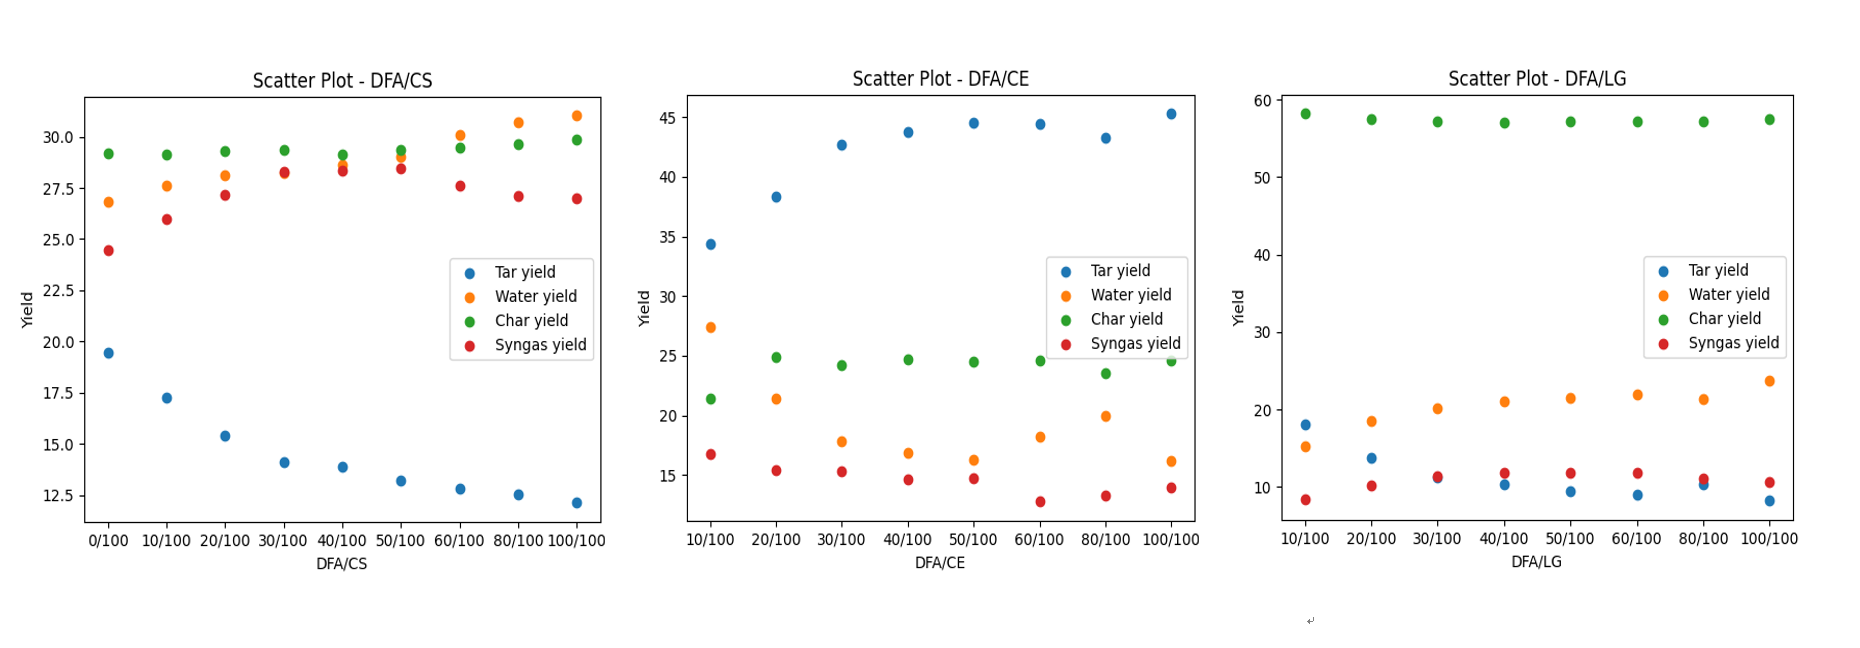
\includegraphics[width=1\linewidth]{./figures/scatter graph.png}}\hfill
    \caption{Scatter plot of the data}
\end{figure}


\section{Assumptions}

To simplify the problem, we make the following assumptions:

\begin{enumerate}
\item The pyrolysis process is a closed system, and the mass of the system is constant.
\item The pyrolysis process is an isothermal process, and the temperature of the system is constant.
\item In formulating the reaction kinetics model, we posit that, during the recorded experimental duration, all reactions have reached complete and thorough completion, and the theoretical premise of cellulose transforming into dehydrated cellulose at low temperatures is valid.
\end{enumerate}

\section{Configuration of Experimental Environment}

All calculations and modeling are conducted within the computational framework of macOS Sonoma 14.1, employing the Apple M2 chip architecture.

The third-party libraries utilized are enumerated in the following table.
\newpage
\begin{table}[h!t]
    \centering
    \caption{third-party libraries}
    \label{tbl:label}
    \begin{tabular}{cccccc}
    \toprule
    package & version  \\
    \midrule
    matplotlib & 3.8.1 \\
    statsmodels & 0.14.0 \\
    scikit-learn & 1.3.2 \\
    scipy & 1.11.3   \\
    \bottomrule
    \end{tabular}
\end{table}

\section{Data visualization and correlation analysis}

In this section, We will visualize the mixing ratio/yield data and perform correlation analysis to determine the impact of the mixing ratio on output.

\subsection{Data visualization}

Use OLS method to fit the data and make a line chart。

\begin{figure}[h!t]
    \centering
    \subfigure{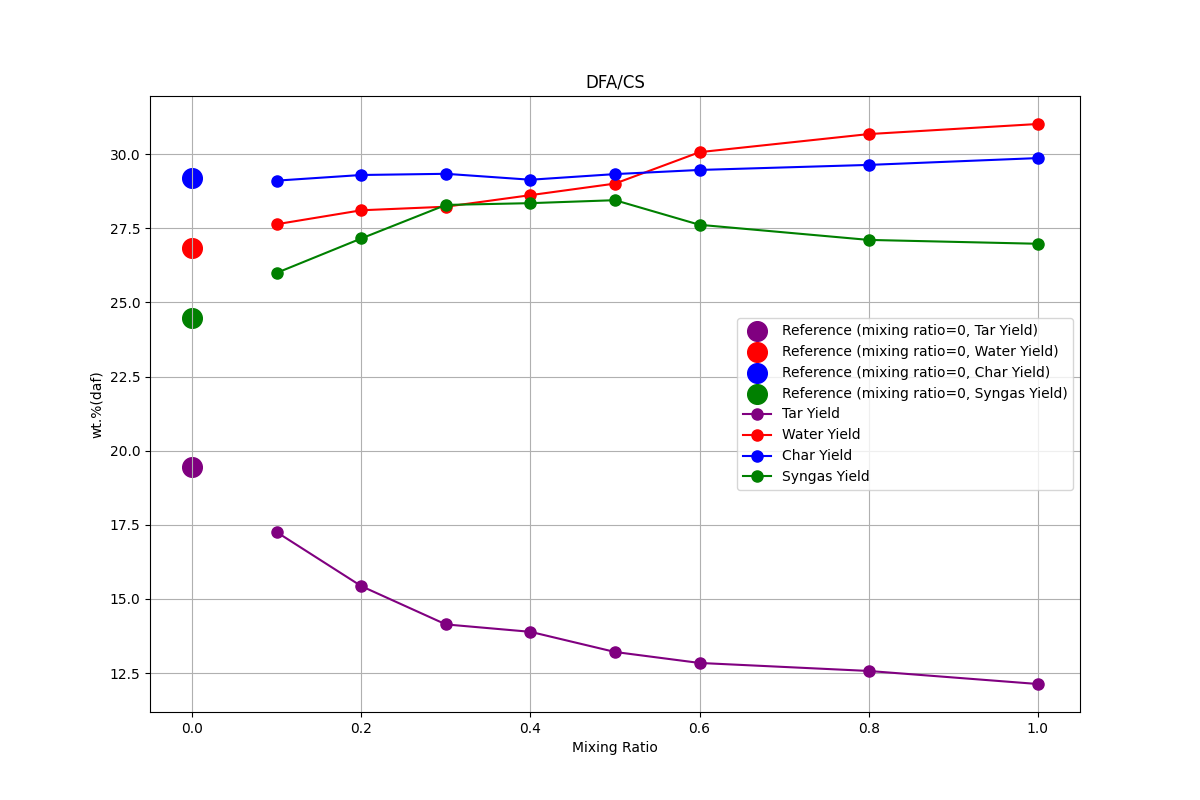
\includegraphics[width=0.95\linewidth]{./figures/linear_regression_DFA_CS.png}}\hfill
    \caption{CS yields}
\end{figure}

\begin{figure}[h!t]
    \centering
    \subfigure{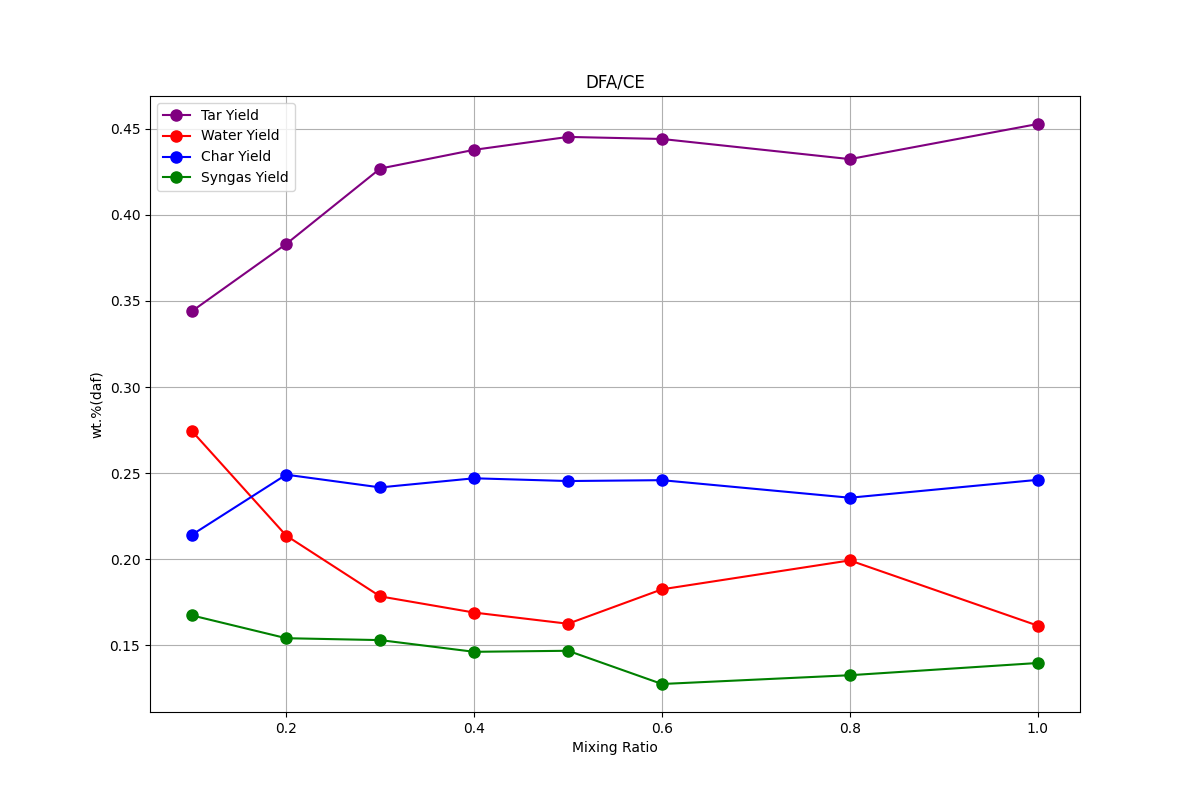
\includegraphics[width=0.95\linewidth]{./figures/linear_regression_DFA_CE.png}}\hfill
    \caption{CE yields}
\end{figure}

\begin{figure}[h!t]
    \centering
    \subfigure{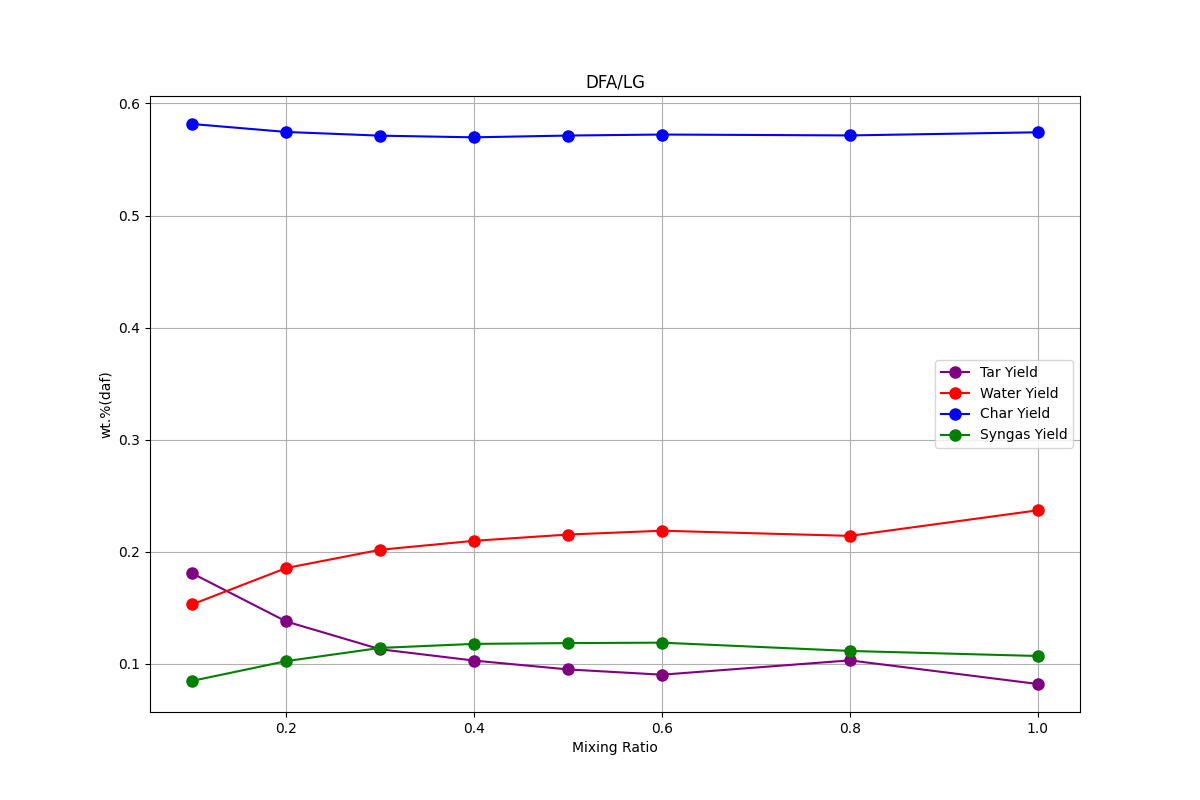
\includegraphics[width=0.95\linewidth]{./figures/linear_regression_DFA_LG.png}}\hfill
    \caption{LG yields}
\end{figure}

It can be seen that the catalyst has an inhibitory effect on cotton stalks (CS) Tar yield, has a relatively large impact on cellulose (CE) Tar yield and water yield, and has basically little impact on lignin (LG).

\subsection{Correlation analysis}

In order to judge the impact of catalysts more scientifically, correlation analysis was conducted.

Judging intuitively from the visual images, the data probably does not satisfy normality, and the sample size is small, so the Kenalltau correlation coefficient is used for analysis.

\begin{figure}[h!t]
    \centering
    \subfigure{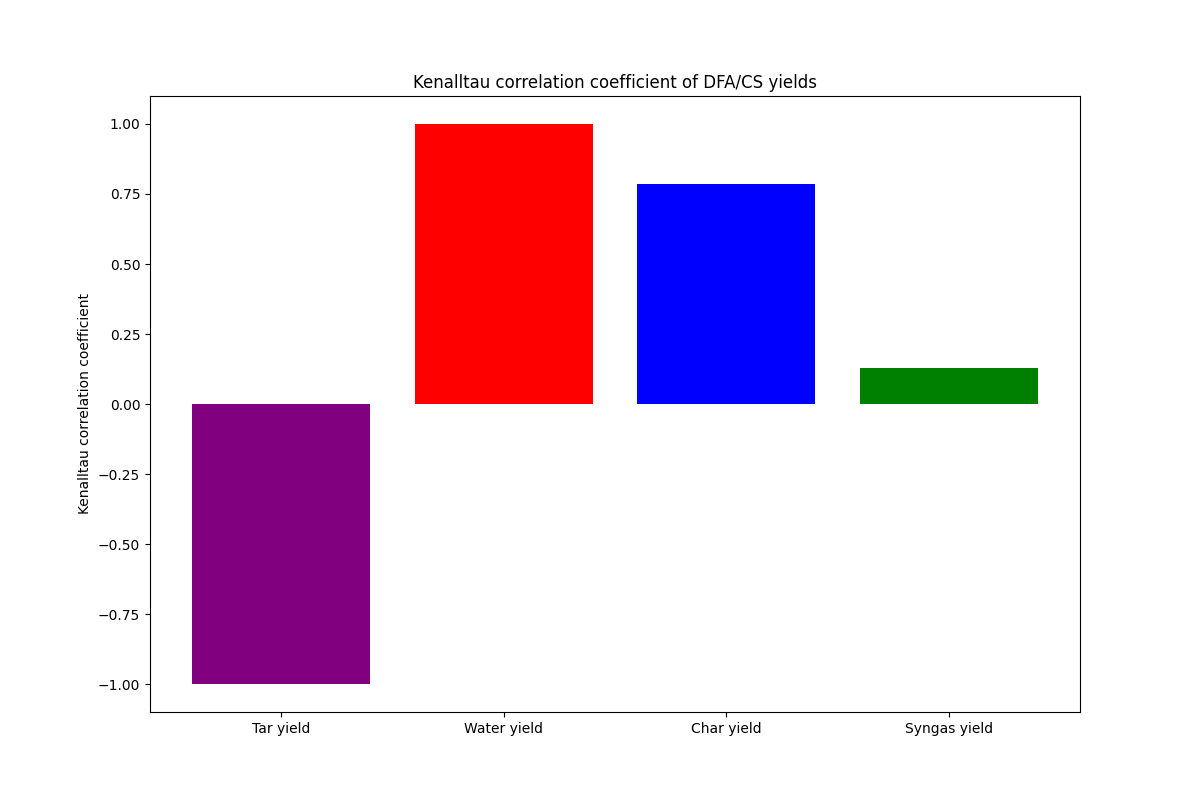
\includegraphics[width=0.65\linewidth]{./figures/Kenalltau_DFA_CS.png}}\hfill
    \caption{Kenalltau correlation coefficient of CS}
\end{figure}

\begin{figure}[h!t]
    \centering
    \subfigure{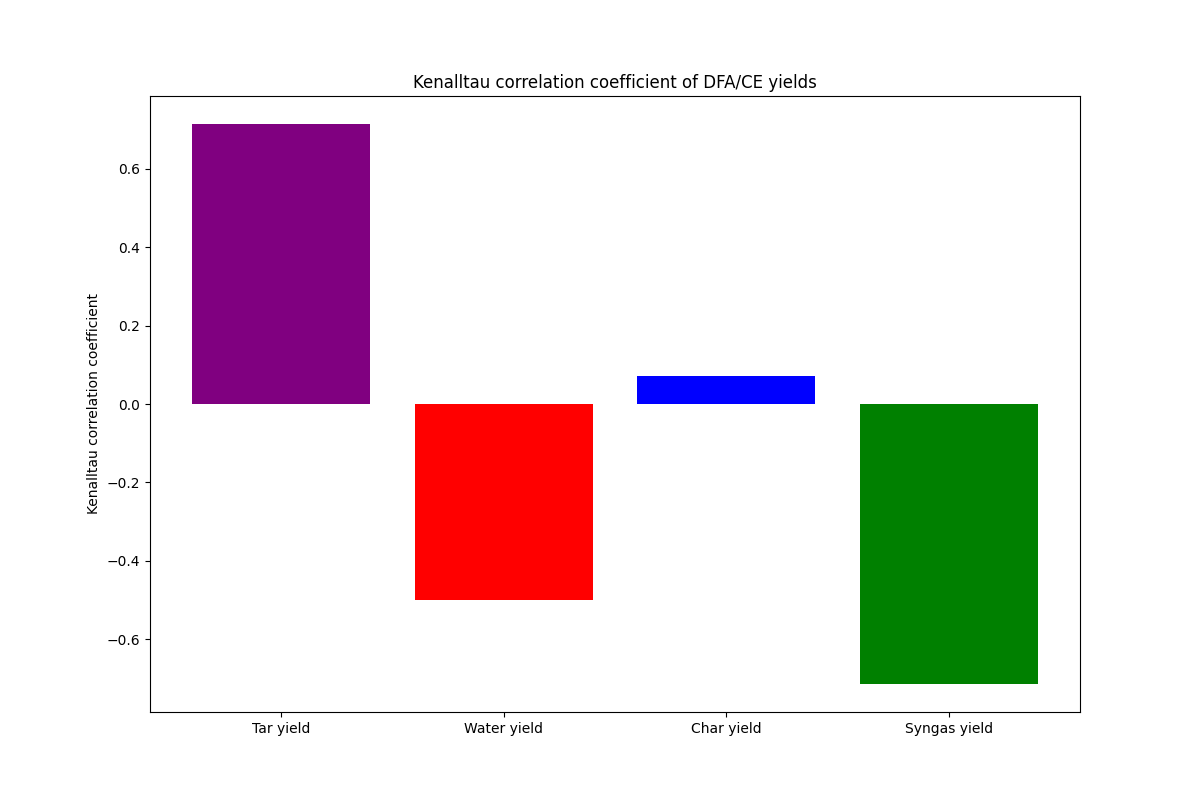
\includegraphics[width=0.65\linewidth]{./figures/Kenalltau_DFA_CE.png}}\hfill
    \caption{Kenalltau correlation coefficient of CE}
\end{figure}

\begin{figure}[h!t]
    \centering
    \subfigure{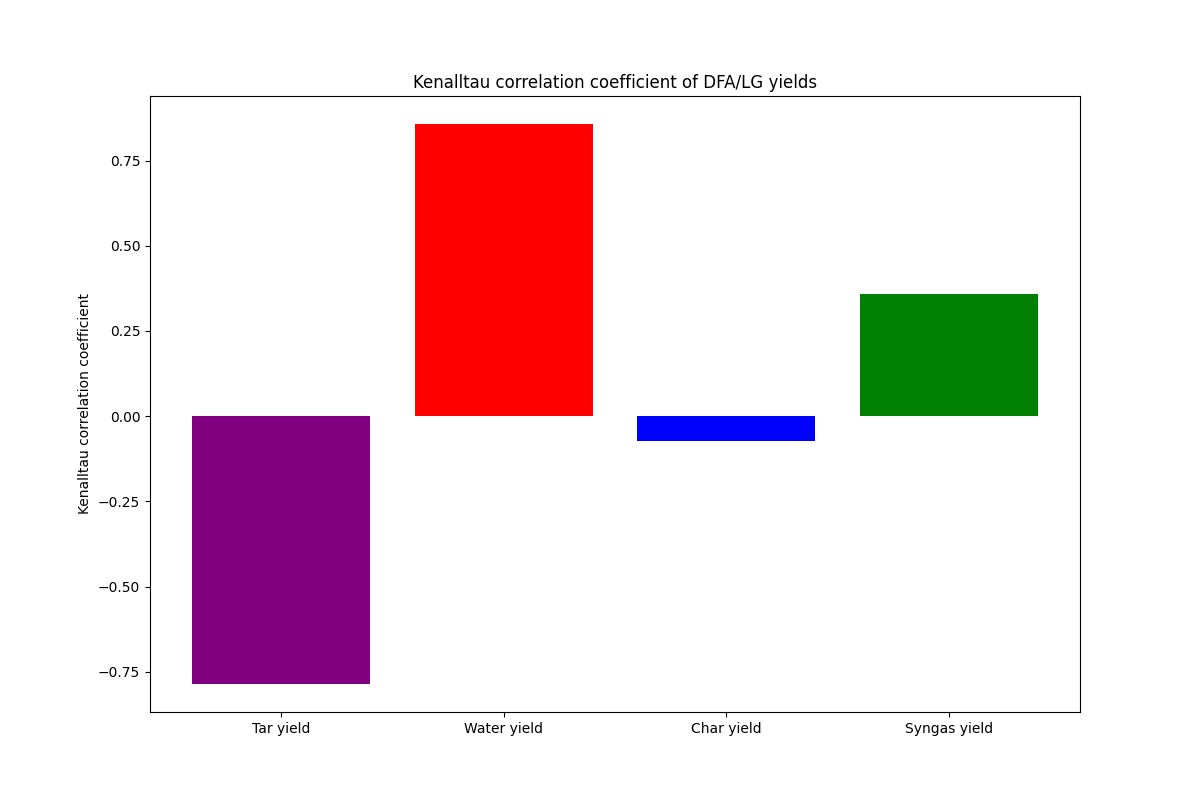
\includegraphics[width=0.65\linewidth]{./figures/Kenalltau_DFA_LG.png}}\hfill
    \caption{Kenalltau correlation coefficient of LG}
\end{figure}

Observations reveal a pronounced positive correlation between the mixing ratio and water yield as well as char yield in the case of cotton stalks (CS), accompanied by a significant negative correlation with tar yield for cotton stalks (CS). Additionally, a robust positive correlation is evident in the case of tar yield for cellulose (CE), while a substantial negative correlation is observed with syngas yield. Likewise, a marked positive correlation is identified with water yield for lignin (LG), coupled with a substantial negative correlation with tar yield.

Furthermore, we calculate the p-value of the test.

\begin{figure}[h!t]   
    \centering
    \subfigure{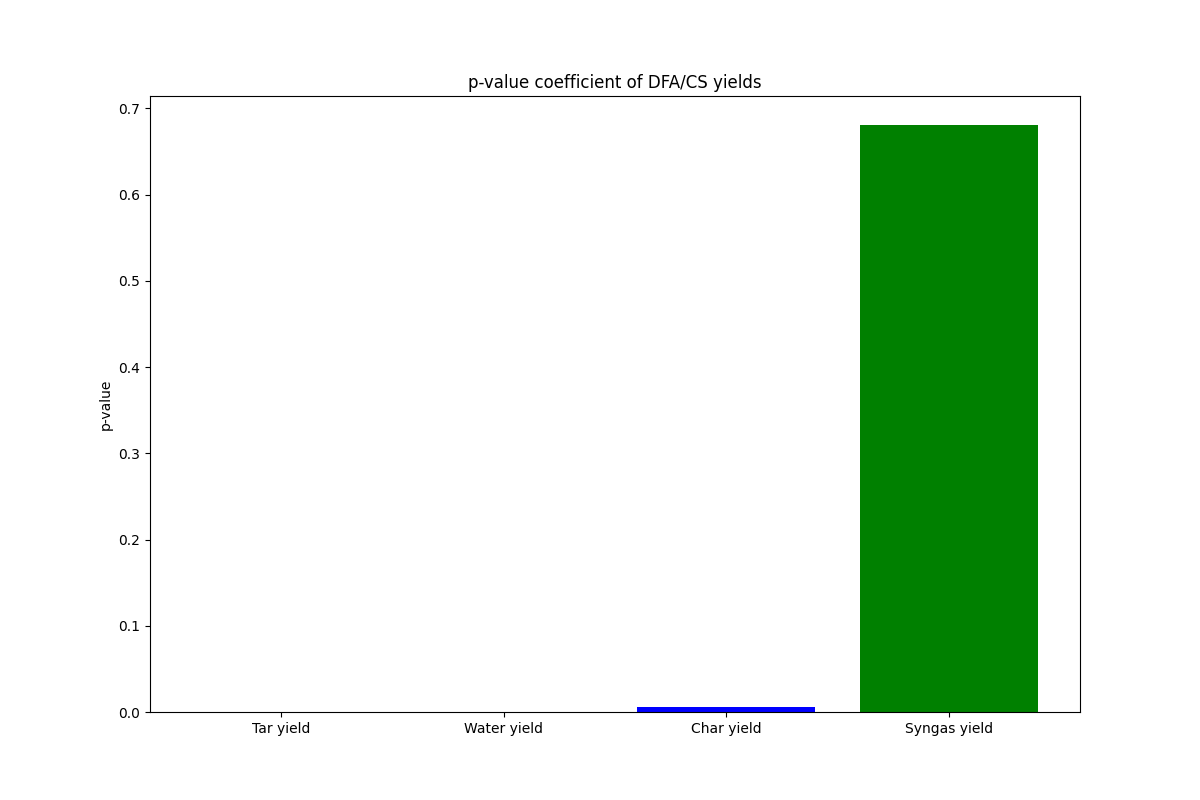
\includegraphics[width=0.85\linewidth]{./figures/p_value_DFA_CS.png}}\hfill
    \caption{p-values in CS}
\end{figure}

\begin{figure}[h!t]
    \centering
    \subfigure{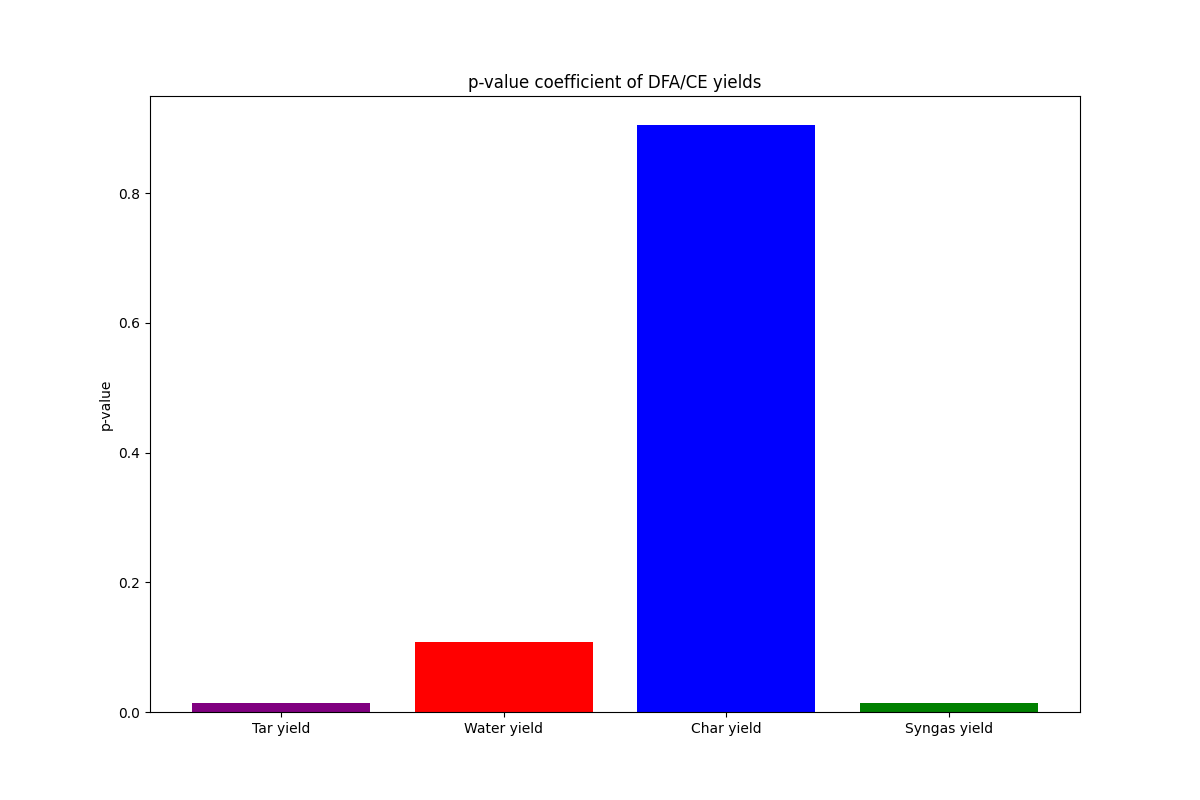
\includegraphics[width=0.85\linewidth]{./figures/p_value_DFA_CE.png}}\hfill
    \caption{p-values in CE}
\end{figure}

\begin{figure}[h!t]
    \centering
    \subfigure{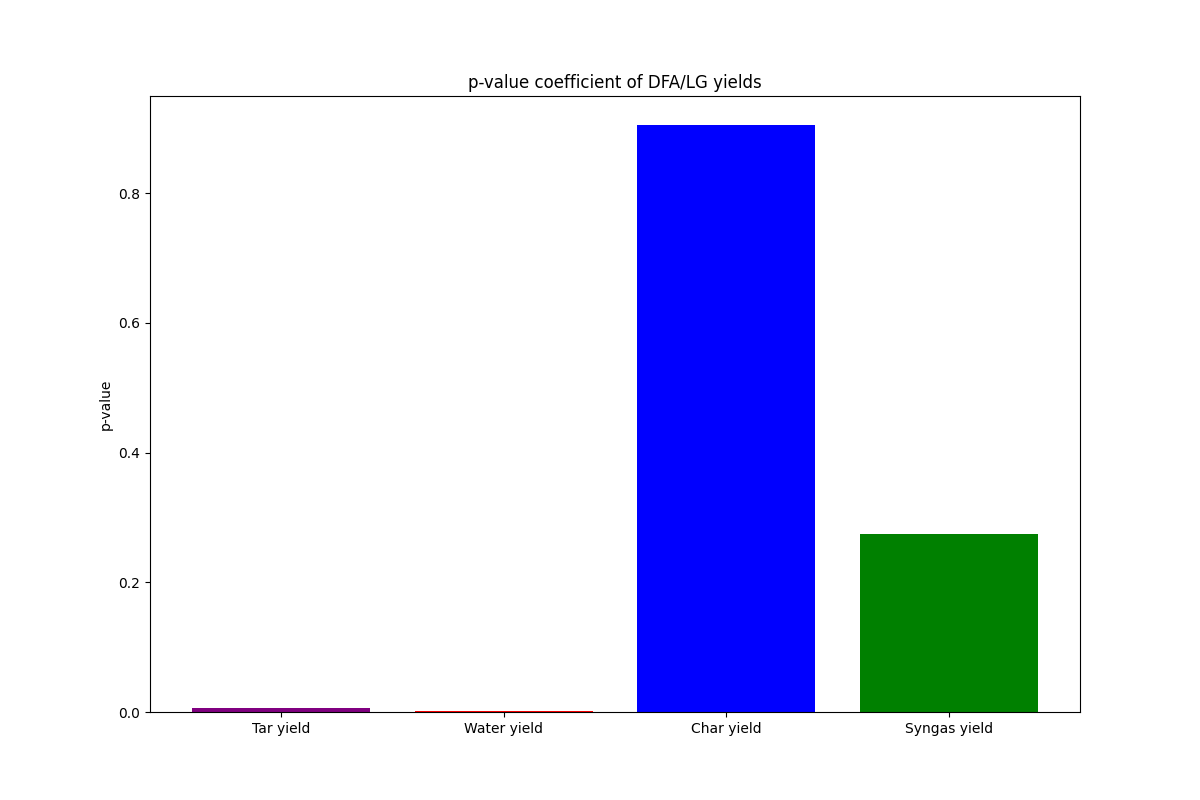
\includegraphics[width=0.85\linewidth]{./figures/p_value_DFA_LG.png}}\hfill
    \caption{p-values in LG}
\end{figure}

Based on the derived p-values, it can be deduced that the catalyst mixing ratio exerts a significant influence on the tar yield, water yield, and char yield of cotton stalks (CS). Additionally, it demonstrates a substantial impact on the tar yield and syngas yield of cellulose (CE), as well as a significant effect on the tar yield and water yield of lignin (LG).

\section{Analysis of Pyrolysis Gas}

We plan to analyze the pyrolysis gas of cotton stalk (CS), cellulose (CE), and lignin (LG) through visual representation techniques.

\subsection{Data visualization}

Visualizations will be conducted utilizing the Matplotlib library.

\begin{figure}[h!t]
    \centering
    \subfigure{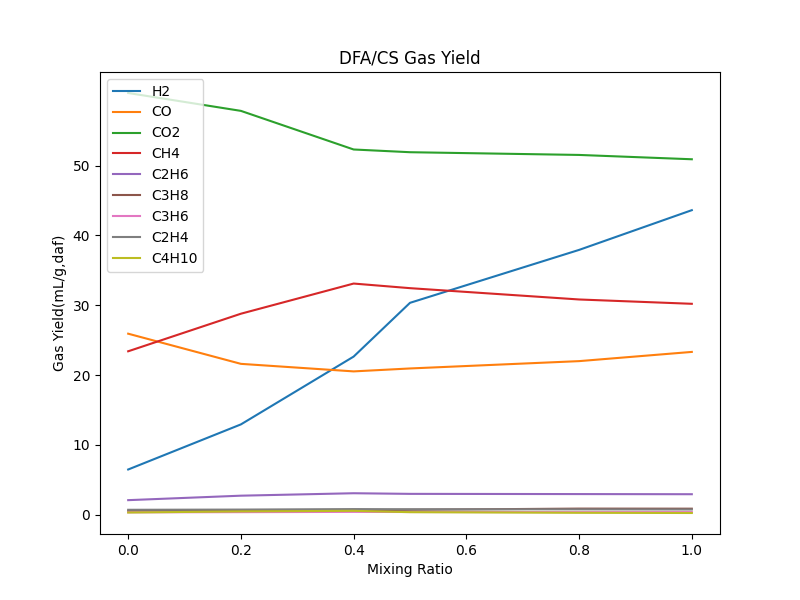
\includegraphics[width=0.65\linewidth]{./figures/DFA_CS_Gas_Yield.png}}\hfill
    \caption{CS gas}
\end{figure}

\begin{figure}[h!t]
    \centering
    \subfigure{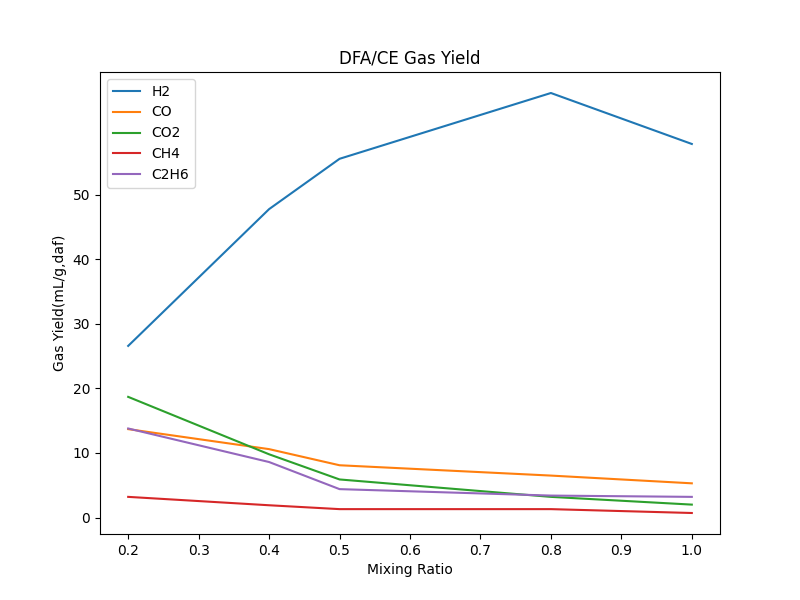
\includegraphics[width=0.65\linewidth]{./figures/DFA_CE_Gas_Yield.png}}\hfill
    \caption{CE gas}
\end{figure}

\begin{figure}[h!t]
    \centering
    \subfigure{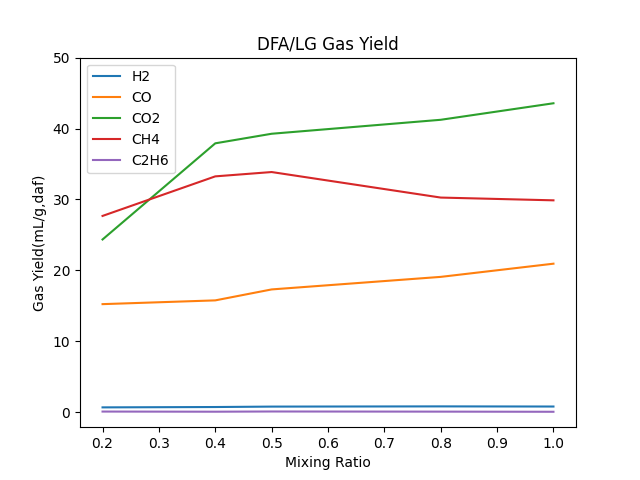
\includegraphics[width=0.65\linewidth]{./figures/DFA_LG_Gas_Yield.png}}\hfill
    \caption{LG gas}
\end{figure}

The visual analysis reveals the following trends:

In the case of cotton stalks (CS) products, those with high carbon content exhibit minimal variation and are generally unaffected by the mixing ratio. Carbon monoxide (CO), carbon dioxide (CO2), and methane (CH4) all exhibit a decline to a certain extent with an increase in the mixing ratio, while hydrogen (H2) demonstrates an increase corresponding to the mixing ratio.

For cellulose (CE) products, there is a notable initial increase followed by a subsequent decrease in hydrogen (H2) yield. Conversely, the yields of other products decrease as the mixing ratio increases.

Contrary to the patterns observed in the first two cases, lignin (LG) products exhibit a lower hydrogen yield, while carbon monoxide (CO), carbon dioxide (CO2), and methane (CH4) yields are higher and show an increasing trend with an elevation in the mixing ratio.

\section{Differential Analysis of Pyrolysis Products}

In this section, a differential analysis will be conducted on the pyrolysis products of cellulose (CE) and lignin (LG) under the same catalyst mixing ratio.

\subsection{Prior to conducting the differential analysis}

Before engaging in differential analysis, an examination of data normality and homogeneity of variance will be carried out to determine the most suitable method for conducting differential analysis.

Due to the relatively small sample size, we will employ tests sensitive to small datasets. Therefore, the assessment of normality will be conducted using the Shapiro-Wilk test, while the evaluation of homogeneity of variance will be performed using the Levene test.

\begin{table}[h!t]
    \centering
    \caption{Shapiro Wilk test}
    \label{tbl:label}
    \begin{tabular}{cccccc}
    \toprule
    yield & p-value & pyrolysis gas & p-value \\
    \midrule
    CE Tar & 0.024 & CE H2 & 0.461 \\
    CE Water & 0.053 & CE CO & 0.767 \\
    CE Char & 0.002 & CE CO2 & 0.353 \\
    CE Syngas & 0.951 & CE CH4 & 0.434  \\
    LG Tar & 0.081 & CE C2H6 & 0.153 \\
    LG Water & 0.325 & LG H2 & 0.452 \\
    LG Char & 0.025 & LG CO & 0.684 \\
    LG Syngas & 0.057 & LG CO2 & 0.102 \\
    & & LG CH4 & 0.591 \\
    & & LG C2H6 & 0.967 \\
    \bottomrule
    \end{tabular}
\end{table}

\newpage

\begin{table}[h!t]
    \centering
    \caption{Levene test}
    \label{tbl:label}
    \begin{tabular}{cccccc}
    \toprule
    CE vs LG & p-value & CE gas vs LG gas & p-value \\
    \midrule
    Tar & 0.804 & H2 & 0.091 \\
    Water & 0.539 & CO & 0.538 \\
    Char & 0.322 & CO2 & 0.965 \\
    Syngas & 0.731 & CH4 & 0.145  \\
    &  & C2H6 & 0.103 \\

    \bottomrule
    \end{tabular}
\end{table}

Through tests, we can see that tar yield and char yield do not satisfy normality.

\subsection{Differential Analysis}

For data that meet the assumptions of normality and homogeneity of variance, an independent samples t-test will be employed. For data that do not meet these assumptions, given the small dataset size, we will utilize the Wilcoxon signed-rank test, which is sensitive to small datasets.

\begin{table}[h!t]
    \centering
    \caption{Levene test}
    \label{tbl:label}
    \begin{tabular}{cccccc}
    \toprule
    Yield & p-value  \\
    \midrule
    Tar & 0.007  \\
    Water & 0.476 \\
    Char & 0.007 \\
    Syngas & 0.00003 \\
    H2 &  0.00007\\
    CO & 0.0013\\
    CO2 &  0.00018 \\
    CH4 &   9.6e-9\\
    C2H6 &  0.011\\

    \bottomrule
    \end{tabular}
\end{table}

The differential analysis reveals significant differences in the product yields of cellulose (CE) and lignin (LG), with the exception of water yield. Particularly notable are the pronounced differences in the levels of syngas, hydrogen (H2), and methane (CH4).

\section{Reaction Mechanism and Kinetics Model}

\subsection{Reaction Mechanism}

We establish catalytic reaction mechanism models for the reactions of cellulose and lignin under the catalysis of desulfurized ash, investigating the catalytic benefits of desulfurized ash on the pyrolysis processes of cellulose and lignin. This analysis is complemented by an examination of the pyrolysis gas distribution maps presented in Section 5.

Concerning the hydrogen content, a notable increase in the hydrogen concentration in the pyrolysis gas components of cellulose is observed with an augmentation in the desulfurized ash content. In contrast, the hydrogen content in lignin reactions remains relatively constant. This suggests that hydrogen predominantly originates from the pyrolysis process of cellulose, and the increase in desulfurized ash content significantly influences the reduction in reaction activation energy for hydrogen production during cellulose pyrolysis. Simultaneously, the reaction hydrogen yield from the desulfurized ash and cotton stalk mixture is lower than that from the cellulose and desulfurized ash mixture, indicating that the combination of lignin and cellulose inhibits the radical reactions responsible for hydrogen generation during cellulose pyrolysis \cite{bib3}.

Concerning the content of carbon monoxide (CO) and carbon dioxide (CO2), the analysis of the graphs indicates that, with an increase in desulfurized ash content, the rates of production for CO and CO2 during cellulose pyrolysis are significantly lower compared to the corresponding gas yields from lignin. This observation suggests that cellulose is not the primary source of CO and CO2, with their predominant generation originating from the pyrolysis of lignin\cite{bib4}.

With the elevation of desulfurized ash content, there is a reduction in the production of carbon monoxide (CO) and carbon dioxide (CO2) during cellulose pyrolysis. Desulfurized ash demonstrates the capacity to inhibit the generation of CO and CO2 in cellulose pyrolysis, and the inhibitory effect becomes more pronounced with higher desulfurized ash content. Concurrently, desulfurized ash also facilitates the production of CO and CO2 during lignin pyrolysis, thereby maintaining relatively stable levels of CO and CO2 in the pyrolysis of cotton stalks. This indicates that, under the catalytic influence of desulfurized ash, the reactions leading to the generation of CO and CO2 during lignin pyrolysis are noticeably promoted, while those associated with cellulose are restrained.

\subsection{Kinetics Model}

During the cellulose pyrolysis process, the initial step involves decrystallization and depolymerization, resulting in the formation of reactive cellulose and dehydrated cellulose. As the temperature increases, the reactive cellulose further decomposes, giving rise to two primary products. The first involves the cleavage of glycosidic bonds, generating products such as levoglucosan. The second entails ring-opening reactions, yielding small molecules like furans, alcohols, and aldehydes. These reactions dominate at low and high temperatures, respectively. Dehydrated cellulose evolves into char and non-condensable gases. Additionally, if the residence time is prolonged, unvolatilized products may undergo polymerization and cleavage, resulting in the formation of char and non-condensable gases. This process is represented by the simplified model depicted in the figure below\cite{bib5}.

\begin{figure}[h!t]
    \centering
    \subfigure{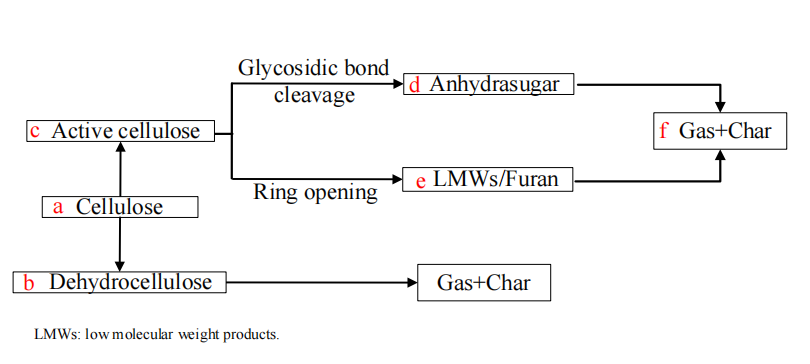
\includegraphics[width=0.8\linewidth]{./figures/kinetic.png}}\hfill
    \caption{kinetic}
\end{figure}

The reaction kinetics modeling analysis is conducted with a heating rate of 30°C/min for the pyrolysis temperature, and the corresponding variation in the weight loss rate is depicted in the graph below.

\begin{figure}[h!t]
    \centering
    \subfigure{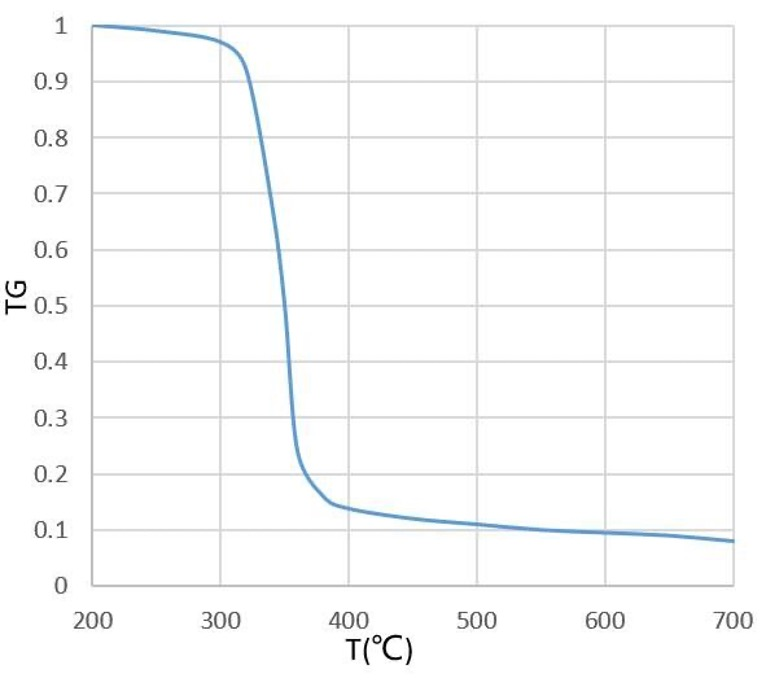
\includegraphics[width=0.63\linewidth]{./figures/TG.jpg}}\hfill
    \caption{TG graph}
\end{figure}

The kinetics equation specifically describing the pyrolysis process is as follows, with the general formulation for solid decomposition reaction kinetics typically expressed as:

\begin{align}
    \label{eq1}
        \frac{d\alpha}{dt} = kf(\alpha)
\end{align}

Moreover, the rate constant K adheres to Arrhenius Law, expressed as:

\begin{align}
    \label{eq2}
        k = Aexp(-\frac{E}{RT})f(\alpha)
\end{align}

Substituting \(k\) into Equation (1) yields Equation (3):

\begin{align}
    \label{eq3}
        \frac{d\alpha}{dt} = Aexp(-\frac{E}{RT})f(\alpha)
\end{align}

In the equation, $f(\alpha)$ represents the reaction mechanism function, where $\alpha$ denotes the conversion rate given by $\alpha = (m_0-m_t)/(m_0-m_{\infty})$, with $m_0, m_t$ and $m_{\infty}$ representing the initial mass, mass at a specific time, and mass when the reaction reaches a stable state, respectively. The variable 
$t$ denotes reaction time in seconds, $A$ epresents the pre-exponential factor in units of $min^{-1}$, $E$ represents the activation energy in kJ/mol, and $R$
is the ideal gas constant (8.3145 J/(mol·K)).

Due to the heating rate $\beta = \frac{dT}{dt}$ and is a constant, and Equation (3) is modified to Equation (4):

\begin{align}
    \label{eq4}
        \frac{d\alpha}{dT} = \frac{A}{\beta}exp(-\frac{E}{RT})f(\alpha)
\end{align}

Define $G(\alpha) = \int_{0}^{\alpha}\frac{d\alpha}{f(\alpha)}$ yielding equation (5).

\begin{align}
    \label{eq5}
    G(\alpha) = \frac{A}{\beta}\int_{0}^{T}exp(-\frac{E}{RT})dT
\end{align}

Differentially or integrally solving Equation (5) to obtain the kinetic parameters is a pivotal step in the process of reaction kinetics modeling analysis.

Presently, the reaction mechanism function that best captures the fitting effectiveness for the cellulose pyrolysis model is the reverse Jander equation\cite{bib6}, expressed as:
$[(1+\alpha)^{\frac{1}{3}}-1]^2$

In this study, the Doyle approximation, \(PD = 0.005 \exp(-1.052u)\), is chosen to replace the temperature integral in the kinetic differential equation, resulting in the final expression:

\begin{align}
    \label{eq6}
    G(\alpha)=\frac{AE}{\beta R}\left(0.005\exp{\left(-1.052\frac{E}{RT}\right)}\right)
\end{align}

From Equation (6), by substituting the reaction mechanism function, the expression for the conversion rate \( \alpha \) under this mechanism can be derived. The thermal weight loss rate of biomass can be represented as:

\begin{align}
    \label{eq7}
    -(\frac{dw}{dt})=   \frac{d\alpha}{dt} \stackrel{\frac{dT}{dt}=\beta}{\longrightarrow} \beta(\frac{d\alpha}{dT})
\end{align}

Consequently, a functional relationship between weight loss rate and reaction temperature can be established, facilitating the analysis of existing data. By employing equations (6) and (7), the expression for the thermal weight loss rate under this mechanistic function can be derived. Nonlinear least squares fitting optimization of the kinetic parameters can be performed using 1StopT software, ultimately yielding the reaction kinetics parameters.

Finally, within the low-temperature range (260°C to 350°C), the pre-exponential factor reference value is determined to be 1.19 multiplied by 10 to the power of 12 per minute, with an activation energy of 154.06 kilojoules per mole. In the high-temperature range (350°C to 400°C), the pre-exponential factor reference value is established as 6.12 multiplied by 10 to the power of 20, with an activation energy reference value of 203.98 kilojoules per mole.

\section{Pyrolysis Prediction Model}

In Section 4, we conducted a preliminary data fitting process. In this subsequent section, an analysis of various conventional mathematical models and AI learning prediction models will be undertaken. The objective is to evaluate the characteristics of these models and choose a suitable approach for the establishment of robust and highly resilient predictive models, given the constraints of limited existing data.

\subsection{Model Selection}

To facilitate prediction, an initial step involves fitting functions to the available data. Various methods exist for function fitting, encompassing linear regression models, polynomial regression models, ridge regression models, support vector regression, decision tree regression, gradient boosting regression, and neural network models. Notably, neural networks, often hailed as "universal function approximators" due to their adeptness at function fitting, are characterized by their opaque nature. However, their efficacy hinges on substantial dataset support, which we lack in this instance, rendering neural network models impractical for our purposes. Consequently, we opt for polynomial regression. This choice is motivated by its heightened sensitivity to small sample sizes and its ability to provide an optimal approximation of the relationship between the dependent and independent variables.

\subsection{Polynomial Regression}


Polynomial regression is an extension of linear regression that allows fitting data using polynomial functions. Its mathematical model can be represented as:

\begin{align}
\label{eq}
    y = \beta_0 + \beta_1 x + \beta_2 x^2 + ... + \beta_n x^n + \epsilon \nonumber
\end{align}

Where:

\begin{itemize}
    \item y is the dependent variable (target variable).
    \item x s the independent variable (input feature).
    \item $\beta_0, \beta_1, ..., \beta_n$ are the coefficients of the model, representing the weights of each term.
    \item n is the degree of the polynomial.
    \item $\epsilon$  is the error term.
\end{itemize}

The principle of polynomial regression involves minimizing the sum of squared residuals, which is the difference between observed values and predicted values. This is typically achieved through the method of least squares, aiming to find coefficients that minimize the sum of squared differences between the model and actual observations.

Advantages of polynomial regression for small-scale data include:

\begin{enumerate}
    \item Polynomial regression is highly flexible and can adapt to various shapes of data, including non-linear relationships.
    \item The coefficients in polynomial regression have an intuitive geometric meaning, with each term representing the impact of the corresponding degree on the curve.
    \item Relative to more complex non-linear models, polynomial regression is relatively easy to understand and interpret.
    \item When there are non-linear relationships in the data, polynomial regression can provide a better fitting effect, accurately reflecting the data's characteristics.
    \item Polynomial regression can be applied to one-dimensional, two-dimensional, or higher-dimensional data, making it suitable for various situations.
\end{enumerate}

\subsection{Establishment of Polynomial Regression Model}

Employing a cubic polynomial regression, we conduct fitting of the function. Using LG's syngas yield as an illustrative example, we generate a graphical representation post-fitting and subsequently extract the model parameters.

\begin{figure}[h!t]
    \centering
    \subfigure{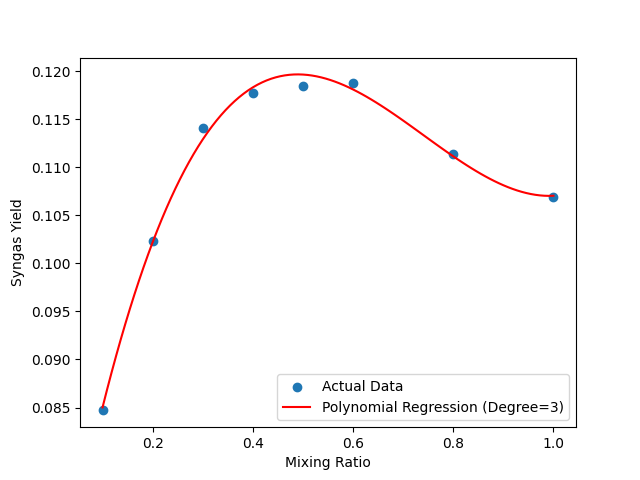
\includegraphics[width=0.65\linewidth]{./figures/poly_regression_syngas.png}}\hfill
    \caption{poly regression of syngas}
\end{figure}

\begin{table}[h!t]
    \centering
    \caption{Model parameters}
    \label{tbl:label}
    \begin{tabular}{cccccc}
    \toprule
    intercept & linear term & quadratic term & cubic term \\
    \midrule
    0.06015761041621481 & 0.29097849 & -0.44394872 & 0.19984241 \\

    \bottomrule
    \end{tabular}
\end{table}

\subsection{Sensitivity Analysis}

Generate validation data to assess the sensitivity, robustness, and resilience of the model.

\begin{figure}[h!t]
    \centering
    \subfigure{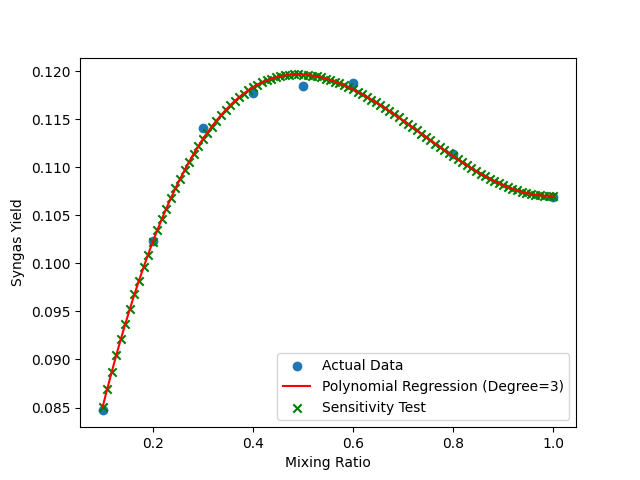
\includegraphics[width=0.65\linewidth]{./figures/check_syngas.png}}\hfill
    \caption{sensitive analysis of syngas}
\end{figure}

It is evident that the model exhibits favorable performance when subjected to validation data. The model established through polynomial regression demonstrates robust performance.

\section{Evaluation and Further Discussion}

\subsection{Strengths}

\begin{itemize}
    \item \textbf{Kinetic}: The Kinetic model detailed consideration of the comprehensive cellulose pyrolysis reaction mechanism, inclusion of quantitative kinetic parameters, and systematic analysis, providing a robust understanding of the process.
    \item \textbf{Polynomial Regression Model}: Its versatility for small-scale data and its ability to accurately capture non-linear relationships. Unlike more complex models, polynomial regression is easy to interpret and adapts well to various data shapes. The cubic polynomial regression, applied to LG's syngas yield, demonstrates the model's effectiveness in approximating complex patterns. The sensitivity analysis further confirms its robust performance with validation data, highlighting its reliability and adaptability for predicting outcomes with limited data. Overall, the model's simplicity, interpretability, and resilience make it a powerful tool for approximating relationships between variables in scenarios with constrained datasets.
\end{itemize}

\subsection{Weakness and Further Discussion}

The weakness of the model lies in its susceptibility to overfitting, especially when dealing with high-degree polynomials. Overfitting occurs when the model fits the training data too closely, capturing noise and idiosyncrasies that do not represent the underlying true pattern in the data. In the context of polynomial regression, higher-degree polynomials introduce more parameters, making the model excessively complex and prone to fitting the noise present in the training data. This complexity may hinder the model's ability to generalize well to new, unseen data, leading to poor predictive performance.

Further discussion on mitigating this weakness involves careful model selection and regularization techniques. Balancing model complexity by choosing an appropriate degree of the polynomial is essential to prevent overfitting. Regularization methods, such as Ridge or Lasso regression, can be employed to penalize overly complex models by adding a regularization term to the objective function. This encourages the model to prioritize simpler solutions, aiding in generalization to new data. Cross-validation techniques can also be utilized to assess model performance on different subsets of the data, helping to identify the optimal level of complexity that minimizes overfitting.

In summary, while polynomial regression offers flexibility, its vulnerability to overfitting underscores the importance of thoughtful model selection and regularization strategies to enhance generalization and predictive accuracy.

%----------------------------参考文献

\begin{thebibliography}{9}%宽度9
\bibitem{bib1} Ming Shan. Current status and challenges of biomass energy development and utilization[J].China Sustainability Tribune,2022(4):48-49
\bibitem{bib2} Libo Zhang, Xintong Dou, Yibo Hao, Keke Zhi, Xuqiang Guo. Characteristics and kinetic analysis of hydrothermal carbon pyrolysis of cotton stalk-based hydrothermal carbon pretreated with different acid and alkali pretreatments[J].Regional Governance,2020(29):0214-0217
\bibitem{bib3} Zhao Jiaxing. Experimental study on the quality improvement of biomass pyrolysis gas phase products by desulfurization ash[D]. Liaoning University of Science and Technology, 2023: 46-52. DOI: 10.26923/d.cnki.gasgc.2022.000413.
\bibitem{bib4} Wang Zexiang, Li Hang, Xie Wenluan, et al. Progress in basic structure, pyrolysis mechanism and characteristics of lignin[J]. New Energy Progress, 2020, 8(01): 6-14.
\bibitem{bib5} Yang Xiaoxiao. Study on the fast pyrolysis mechanism of cellulose based on typical products and construction of a model[D]. Beijing Forestry University, 2021: 55-64. DOI: 10.26949/d.cnki.gblyu.2020.000093.
\bibitem{bib6} Bai Bin, Zhou Weihong, Ding Yifei, et al. Study on kinetic analysis methods of cellulose pyrolysis[J]. Biomass Chemical Engineering, 2017, 51(04): 8-16.
\end{thebibliography}

% ---------------------开始附录


% ----------------
% 在目录中添加格式规范,可以删掉

% \section*{Format specification}
%\addcontentsline{toc}{section}{Format specification}
%
%\includepdfmerge{2023shuweibei,1-3}

\end{document} 